% ============================================================
%  main.tex  —  Collector Premiums and the Wine Life-Cycle
%  Author : Juan F. Imbet
%  Date   : 2026-03-29
%  NOTE   : This is the Overleaf-ready copy. Do NOT edit here.
%           Edit paper/main.tex and run /migrate-overleaf to sync.
%           Coauthors: edit model.tex (top-level) for the model section.
% ============================================================

\documentclass[12pt]{article}

% ── Packages ─────────────────────────────────────────────────────────────────
\usepackage[margin=1in]{geometry}
\usepackage{amsmath,amssymb}
\usepackage{booktabs}
\usepackage{threeparttable}
\usepackage{graphicx}
\usepackage{natbib}
\usepackage{hyperref}
\usepackage{setspace}
\usepackage{caption}
\usepackage{subcaption}
\usepackage[nolists,tablesfirst]{endfloat}

\hypersetup{
  colorlinks = true,
  linkcolor  = blue,
  citecolor  = blue,
  urlcolor   = blue
}

\doublespacing

% ── Theorem environments ──────────────────────────────────────────────────────
\usepackage{amsthm}
\newtheorem{proposition}{Proposition}
\newtheorem{lemma}{Lemma}
\newtheorem{assumption}{Assumption}

% ── Title ─────────────────────────────────────────────────────────────────────
\title{\textbf{Liquid Assets}\thanks{%
         We thank Lucie Bourdychova and Xin Ning for excellent research assistance.
         All errors are our own.}}

\author{Juan F.\ Imbet\thanks{Paris Dauphine University -- PSL.
         \texttt{juan.imbet@dauphine.psl.eu}.} \and
        Roman Kr\"{a}ussl\thanks{Bayes Business School, City St George's University of London.} \and
        Ilaria Piatti\thanks{Queen Mary University of London.} \and
        Roberto Steri\thanks{University of Luxembourg.}}

\date{March 2026}

% ── Document ─────────────────────────────────────────────────────────────────
\begin{document}

\maketitle

{\singlespacing
\begin{abstract}
  Using a panel of 1,068,703 French fine-wine auction transactions (1996--2015), we document
  that the price-age profile of top wines is non-monotone: prices rise through the pre-maturity
  period, peak near the maturity threshold, dip by 26\,\% in the post-maturity trough zone
  (approximately 32--40 years of age), and recover to a collector premium at antique ages.
  The dip is present for Bordeaux Crus Class\'es and Burgundy Premier Cru but absent for
  Burgundy Grand Cru, whose median young-wine price (\$213 per bottle) screens out consumption
  buyers from the outset. We develop a two-type structural demand model in which collectors
  and consumption buyers have heterogeneous valuations for aged wines; the exit of consumption
  buyers at peak maturity creates a temporary oversupply that depresses prices, and only wines
  with a sufficiently high collector-segment share avoid the trough. We estimate the model
  structurally, recovering buyer-type shares and valuation parameters, and find that the
  collector share rises sharply post-maturity, rationalizing both the price dip and the
  antique-age recovery.
\end{abstract}
}

\bigskip

\noindent\textbf{JEL Codes:} G12, D44, L66\\
\noindent\textbf{Keywords:} wine, auction prices, collector premium, maturity, alternative investments

\newpage

% ── Sections ─────────────────────────────────────────────────────────────────
% ============================================================
%  Section 1 — Introduction
% ============================================================

\section{Introduction}
\label{sec:intro}

Fine wine is unusual among investment assets because it ages out. A bottle has a biological
maturity date past which its consumption value declines, yet its market price need not follow
suit: collectors bid for old wine precisely because it can no longer be drunk in the ordinary
sense. This paper uses a large panel of French fine-wine auction transactions to study how
prices evolve over the wine life-cycle, and to show that the shape of the price-age profile
reveals the composition of demand.

\noindent\textit{[Opening paragraph: motivate the puzzle more sharply — most assets appreciate
or depreciate monotonically; wine does neither. Frame the maturity date as the key object:
it creates a natural experiment in which the same bottle transitions from a consumption good
to a collectible in real time.]}

Using 1,068,703 lot-level hammer prices from French fine-wine auctions (1996--2015), we
document a striking non-monotonicity in the price-age profile of premier-quality wines.
Prices rise through the pre-maturity period, peak near the biological maturity window, then
\textit{dip} by approximately 26 percent in a ``trough zone'' spanning the decade after
peak maturity, before recovering to a collector premium at antique ages. This three-phase
pattern is pervasive for Bordeaux Crus Class\'es and Burgundy Premier Crus but is
\textit{absent} for Burgundy Grand Crus, whose auction prices rise monotonically through
the entire life-cycle.

The divergence between Bordeaux and Burgundy Grand Cru identifies the mechanism.
Among young lots (below eight years old), 51.5 percent of Burgundy Grand Cru transactions
exceed \$200 per bottle, compared with 39.0 percent for Bordeaux Crus Class\'es and only
11.2 percent for Burgundy Premier Cru. The high entry price of Burgundy Grand Cru screens
out consumption buyers from the outset: a bidder who intends to drink the wine must be
willing to pay collector-level prices even when the wine is young. There is no consumption
demand segment to exit at peak maturity, and therefore no downward price pressure in the
trough zone.

To formalise this logic, we develop a parsimonious two-type auction model following
\citet{lovo2018}. Buyers are either consumption buyers, who value the wine for drinking
(and whose valuation peaks at maturity and declines thereafter), or collector buyers, who
place an increasing value on rarity and age. The model predicts a non-monotone price-age
profile whenever the consumption-buyer valuation at maturity exceeds the collector-buyer
floor, and a monotone profile when the collector floor is sufficiently high. Three
propositions characterise (i) existence of the non-monotone profile, (ii) the conditions
for trough disappearance, and (iii) comparative statics on trough depth.

Our paper relates to two strands of literature. The first is the empirical literature on
alternative assets as investments \citep{baumol1986, goetzmann1993, mei2002,
korteweg2016, goetzmann2021}. Within this strand, the closest paper is
\citet{dimson2015}, who use a repeat-sales index constructed from Bordeaux Premiers Crus
hammer prices over 1900--2012 to estimate a net real return to wine of 4.1\,\% per annum
and document that young maturing wines generate the highest returns while past-maturity
ch\^{a}teaux provide growing non-pecuniary (collector) benefits. Our paper departs from
\citet{dimson2015} in three important ways. First, they use raw calendar age and therefore
conflate wines at very different stages of their biological life-cycle: a twenty-year
Bordeaux Premier Cru may be at peak maturity while a twenty-year village wine is already in
the trough zone. We normalise age by each wine's individual maturity date, obtained from
Tastingbook for 75.9\,\% of lots and imputed otherwise, which maps heterogeneous calendar
ages onto a common life-cycle grid and isolates the maturity transition as the key event.
Second, the repeat-sales method used in \citet{dimson2015} requires a bottle to be resold
at least twice and therefore systematically excludes the most illiquid segments of the
market; our lot-level panel is ten times larger and covers three wine regions. Third, and
most importantly, \citet{dimson2015} characterise the maturity kink descriptively but do not
model the mechanism. The decomposition of the price dip into a buyer composition effect ---
the exit of consumption buyers at peak maturity --- and the ensuing recovery as collectors
dominate antique-age auctions requires a structural model with heterogeneous buyer types,
which we provide. \citet{breeden2017} use age-period-cohort decomposition on 1.5 million
auction records and confirm the three-phase price profile, but likewise stop short of
modelling why the dip is present for some wine categories and absent for others.

The second strand is the theory of heterogeneous-buyer markets for durable goods. The
structural model of \citet{lovo2018} is our closest theoretical antecedent. They develop
a two-type framework for the art market in which an asset is held by either a ``pleasure
buyer'' (who derives a flow utility from ownership) or a ``speculative buyer'' (who holds
it purely for resale). Their key result is that speculation generates price cycles and
excess volatility relative to fundamental value. Our model shares the two-type architecture
but differs in a central respect: \textit{wine has a finite consumption life}. We model the
consumption-buyer valuation as single-peaked at the maturity date and declining thereafter
--- a restriction that has no counterpart in \citet{lovo2018}, where the pleasure buyer's
flow utility is constant and the asset never expires. It is precisely this biological
maturity structure that generates the non-monotone price-age profile and the composition
effect at the heart of our analysis. A second difference is institutional: wine is sold in
one-shot Vickrey auctions rather than in a search-and-matching market, which allows us to
derive the equilibrium price in closed form and take it directly to data. The maturity
date also provides a natural source of cross-sectional variation to identify the model: the
same wine category at the same calendar age can be pre-maturity or post-maturity depending
on the wine's individual $\tau_i$, and this variation is observable.

\noindent\textit{[Roadmap paragraph: Section~\ref{sec:data} describes the data.
Section~\ref{sec:empirics} presents the empirical strategy. Section~\ref{sec:results} reports
results. Section~\ref{sec:model} develops the structural model that rationalises these
findings. Section~\ref{sec:conclusion} concludes.]}

% ============================================================
%  Section 2 — Data
% ============================================================

\section{Data}
\label{sec:data}

\subsection{Auction transactions}

Our primary dataset consists of lot-level hammer prices from French fine-wine auctions covering
the period 1996--2015. Each observation records the château or domaine, vintage year, bottle
format, auction house, sale date, and realised price per bottle in USD. After applying the
sample selection criteria described below, the working sample comprises 1,068,703 lots.
We restrict attention to three regions: Bordeaux (615,078 lots), Burgundy (328,371 lots), and
the Rhône Valley (105,450 lots).

\subsection{Sample selection}
\label{sec:data:selection}

We apply the following sequential exclusions to arrive at the analysis sample:

\begin{enumerate}
  \item \textbf{Non-positive prices.} We drop lots with a hammer price at or below zero
        (data-entry errors and passed lots recorded as zero). \textit{[Report count dropped.]}
  \item \textbf{Non-standard bottle formats.} We retain only standard (750\,ml) and
        magnum (1.5\,L) formats; jeroboams and larger are excluded because their price-per-bottle
        series is thin and driven by different demand. \textit{[Report count dropped.]}
  \item \textbf{Mixed lots.} Lots containing more than one châteu or vintage within the same
        hammer price are flagged and excluded, as the per-bottle price cannot be attributed to a
        single wine. \textit{[Report count dropped.]}
  \item \textbf{Extreme price outliers.} \textit{[Describe outlier trimming rule, if any —
        e.g., top/bottom 0.1\% of log prices within region-vintage cells.]}
  \item \textbf{Vintage range.} We restrict to vintages 1950--2014 to ensure at least one
        year of auction history and exclude pre-Phylloxera vintages for which maturity data
        are unavailable. \textit{[Confirm exact vintage cutoffs.]}
\end{enumerate}

\noindent Table~\ref{tab:full_sample} in Appendix~\ref{app:full_sample} reports lot counts
and median prices for the full pre-exclusion sample broken down by region and wine type.
\textit{[Add an attrition table showing the count at each exclusion step.]}

\subsection{Maturity windows from Tastingbook}
\label{sec:data:tastingbook}

A central feature of our approach is that maturity dates vary across wines: a top Bordeaux
Cru Classé may peak at 25--30 years after vintage, while a lighter Burgundy village wine may
peak at 8--12 years. Treating all wines as maturing on the same calendar would conflate wines
at very different points in their life-cycles. We therefore match each auction lot to a
wine-specific maturity window.

We match auction lots to drink windows from Tastingbook, a comprehensive online
cellar-management database maintained by professional sommeliers and oenologists.
For each château--vintage pair, Tastingbook records a ``drink-from'' year and a
``drink-until'' year; we define the maturity peak $\tau_i$ as the midpoint of this window,
measured in years since the vintage.
\textit{[Add a sentence or two about the scraping procedure and coverage — how many
châteaux-vintages are in Tastingbook, how we matched to auction records (on château name
and vintage year), and any name-standardisation steps.]}

We match 75.9\,\% of auction lots to a Tastingbook record. For the remaining 24.1\,\%, we
impute $\tau_i$ using a gradient-boosting model trained on the matched observations
(cross-validated $R^2 = 0.991$; see Appendix~\ref{app:imputation}). Features for
imputation include the producer, appellation, region, grape variety, and vintage year.

All maturity values are capped at 20 years. Tastingbook recommendations for old vintages
sometimes anchor to the current date (``drink now''), inflating years-to-maturity to
implausible values; 20 years is a conservative and defensible upper bound given the
sample period and the distribution of grand cru maturities.
\textit{[Consider adding a figure showing the distribution of $\tau_i$ across wine types,
illustrating the cross-sectional variation that powers our identification.]}

\subsection{Normalised age}

We normalise wine age by the wine-specific maturity calendar. Define
\begin{equation}
  a_{it}^* = \frac{t - v_i}{\tau_i},
  \label{eq:age_norm}
\end{equation}
where $t$ is the sale year, $v_i$ is the vintage year, and $\tau_i$ is the maturity-peak
year. By construction $a_{it}^* = 1$ when the wine is sold exactly at its maturity peak;
$a_{it}^* < 1$ indicates pre-maturity and $a_{it}^* > 1$ indicates post-maturity. Across
all lots, 72.3\,\% are sold pre-maturity, consistent with speculative and investment demand
dominating auction supply.

\subsection{Grand cru subsamples}

Our main analysis focuses on the highest-quality wines, where the consumer/collector distinction
is sharpest. We define three groups:

\begin{enumerate}
  \item \textbf{Bordeaux Crus Classés (red):} all classified growths from the Médoc, Graves,
        and Saint-Émilion (436,413 lots).
  \item \textbf{Burgundy Grand Cru:} all Grand Cru appellations from the Côte d'Or (221,512 lots).
  \item \textbf{Burgundy Premier Cru:} all Premier Cru appellations from the Côte d'Or
        (87,136 lots).
\end{enumerate}

Summary statistics for these groups are reported in Table~\ref{tab:summary_stats}.

% ============================================================
%  Section 4 — Empirical Strategy
% ============================================================

\section{Empirical Strategy}
\label{sec:empirics}

\subsection{Price-age profile}

We characterise the price-age profile non-parametrically using a natural cubic spline
regression. Let $p_{it}$ denote the log price per bottle (USD) for lot $i$ sold at time $t$.
We estimate:
\begin{equation}
  p_{it} = f(a_{it}^*) + \varepsilon_{it},
  \label{eq:spline}
\end{equation}
where $f(\cdot)$ is a natural cubic spline with five interior knots at $a^* \in
\{0.4, 0.8, 1.2, 1.6, 2.2\}$, fitted separately for each group. We report predicted
log prices and 95\,\% confidence bands on a fine grid over $a^* \in [0.05, 2.9]$.
Standard errors are heteroskedasticity-robust (HC1).

\subsection{Testing the post-maturity dip}

To formally test whether prices dip below the peak-maturity level in the post-maturity period,
we define five age-norm segments and estimate:
\begin{equation}
  p_{it} = \alpha + \sum_{s \neq \text{young}} \beta_s \mathbf{1}[a_{it}^* \in S_s] + \varepsilon_{it},
  \label{eq:segments}
\end{equation}
where the segments are: \textit{young} $[0, 0.6)$, \textit{approach} $[0.6, 1.0)$,
\textit{peak} $[1.0, 1.6)$, \textit{trough} $[1.6, 2.0)$, and \textit{antique} $[2.0, 3.0]$.
The coefficient of interest is the direct contrast $\beta_{\text{trough}} - \beta_{\text{peak}}$,
tested one-sided (trough $<$ peak). We compute this contrast and its standard error from the
estimated covariance matrix of~\eqref{eq:segments}.

\subsection{Wine-specific maturity normalisation: identification from cross-wine variation}
\label{sec:empirics:normalisation}

A key feature of our design is that $\tau_i$ varies across château--vintage pairs,
creating within-region cross-sectional variation in maturity dates. A 1990 Pétrus (with
$\tau_i \approx 30$ years) and a 1990 Pomerol village wine (with $\tau_i \approx 12$ years)
are both sold in 2005 at calendar age 15, but their normalised ages differ markedly:
$a^* = 0.50$ versus $a^* = 1.25$. Using raw calendar age would conflate pre-maturity
speculation in the Pétrus with post-maturity discounting in the village wine.

The normalisation in equation~\eqref{eq:age_norm} maps both bottles onto the same
life-cycle grid. The identifying assumption is that the per-unit-of-normalised-age
price path is the same across wines within a category, conditional on $a^*$. This is
testable: we verify that the spline fit is stable across terciles of $\tau_i$ within
each wine group. \textit{[Add robustness: estimate equation~\eqref{eq:spline} separately for
wines with low, medium, and high maturity dates; show that the normalised profiles overlap.]}

\subsection{Piecewise linear robustness}
\label{sec:empirics:piecewise}

As a complement to the non-parametric spline, we estimate a piecewise linear specification
with breakpoints at maturity ($a^* = 1.0$) and at the antique threshold ($a^* = 2.0$):
\begin{equation}
  p_{it} = \alpha + \beta_1 a_{it}^* + \beta_2 (a_{it}^* - 1)_+ + \beta_3 (a_{it}^* - 2)_+
           + \varepsilon_{it},
  \label{eq:piecewise}
\end{equation}
where $(x)_+ \equiv \max(0,x)$. The slope in each zone is:
pre-maturity $\beta_1$; trough zone $\beta_1 + \beta_2$; antique $\beta_1 + \beta_2 + \beta_3$.
A negative trough slope ($\beta_1 + \beta_2 < 0$) directly implies that prices \emph{decline}
with age in the post-maturity period, consistent with the non-monotone profile.
Standard errors are heteroskedasticity-robust (HC1); the trough slope is computed by the
delta method.

\subsection{Fixed effects specifications}
\label{sec:empirics:fe}

The baseline specifications~\eqref{eq:segments} and~\eqref{eq:piecewise} do not include
producer or vintage fixed effects. The market-level price-age profile is the target estimand:
how auction prices for these wine categories move over the life-cycle on average. Producer
demeaning would absorb between-producer variation that is part of the mechanism — as wines age
into the trough zone, the cross-sectional mix of producers shifts toward lower-prestige bottles,
because top producers' wines are withheld from the market longer. That compositional shift is
the mechanism we want to document, not a nuisance to partial out.

Nevertheless, as a robustness check we report specifications that absorb vintage year fixed
effects (to control for cohort quality differences) and producer fixed effects. The segment
coefficients in those specifications identify within-vintage and within-producer price-age
patterns. If the trough is a genuine life-cycle phenomenon rather than a selection artifact,
it should survive both sets of fixed effects.

\subsection{Robustness and identification}
\label{sec:empirics:robust}

\noindent\textit{[To be completed. Planned robustness checks:]}
\begin{itemize}
  \item \textit{Alternative knot placements for the spline (3, 7, and 9 interior knots).}
  \item \textit{Polynomial alternatives (cubic and quartic in $a^*$).}
  \item \textit{Vintage-year fixed effects to absorb cohort quality differences.}
  \item \textit{Auction-house fixed effects.}
  \item \textit{Separate estimates for bottle vs.\ magnum formats.}
  \item \textit{Robustness of segment boundaries in equation~\eqref{eq:segments}
        (shift trough window to $[1.5, 2.0)$ and $[1.6, 2.2)$).}
  \item \textit{Results stratified by low/medium/high maturity tercile to validate
        the normalisation assumption.}
\end{itemize}

% ============================================================
%  Section 5 — Results
% ============================================================

\section{Results}
\label{sec:results}

\subsection{The price-age profile: Bordeaux vs.\ Burgundy}

Figure~\ref{fig:spline} plots the estimated natural cubic spline for all six groups against
normalised wine age. Panels~A and~B display the Bordeaux and Burgundy subgroups separately;
Panel~C juxtaposes the aggregate Bordeaux and Burgundy series. Through the pre-maturity period,
log prices rise monotonically for all groups — that much is uncontroversial. The divergence
comes after maturity.

Among Bordeaux wines, both the Grand Cru tier (1\textsuperscript{er} Cru Class\'es M\'edoc and
Premiers grands crus class\'es A, St\'emilion) and the Premier Cru tier (2\textsuperscript{nd}
through 5\textsuperscript{th} growths plus Graves and St\'emilion~B) exhibit a pronounced dip in
the trough zone ($a^* \in [1.6, 2.0)$, approximately 32--40 years of age). The Bordeaux Grand
Cru dip is the deepest, consistent with the longer maturity windows and higher consumption
valuations at peak for the most prestigious châteaux. Among Burgundy wines, Burgundy Grand Cru
continues to rise through the same window without interruption; Burgundy Premier Cru shows a
mild inflection but no sustained decline.

\begin{figure}[htbp]
  \centering
  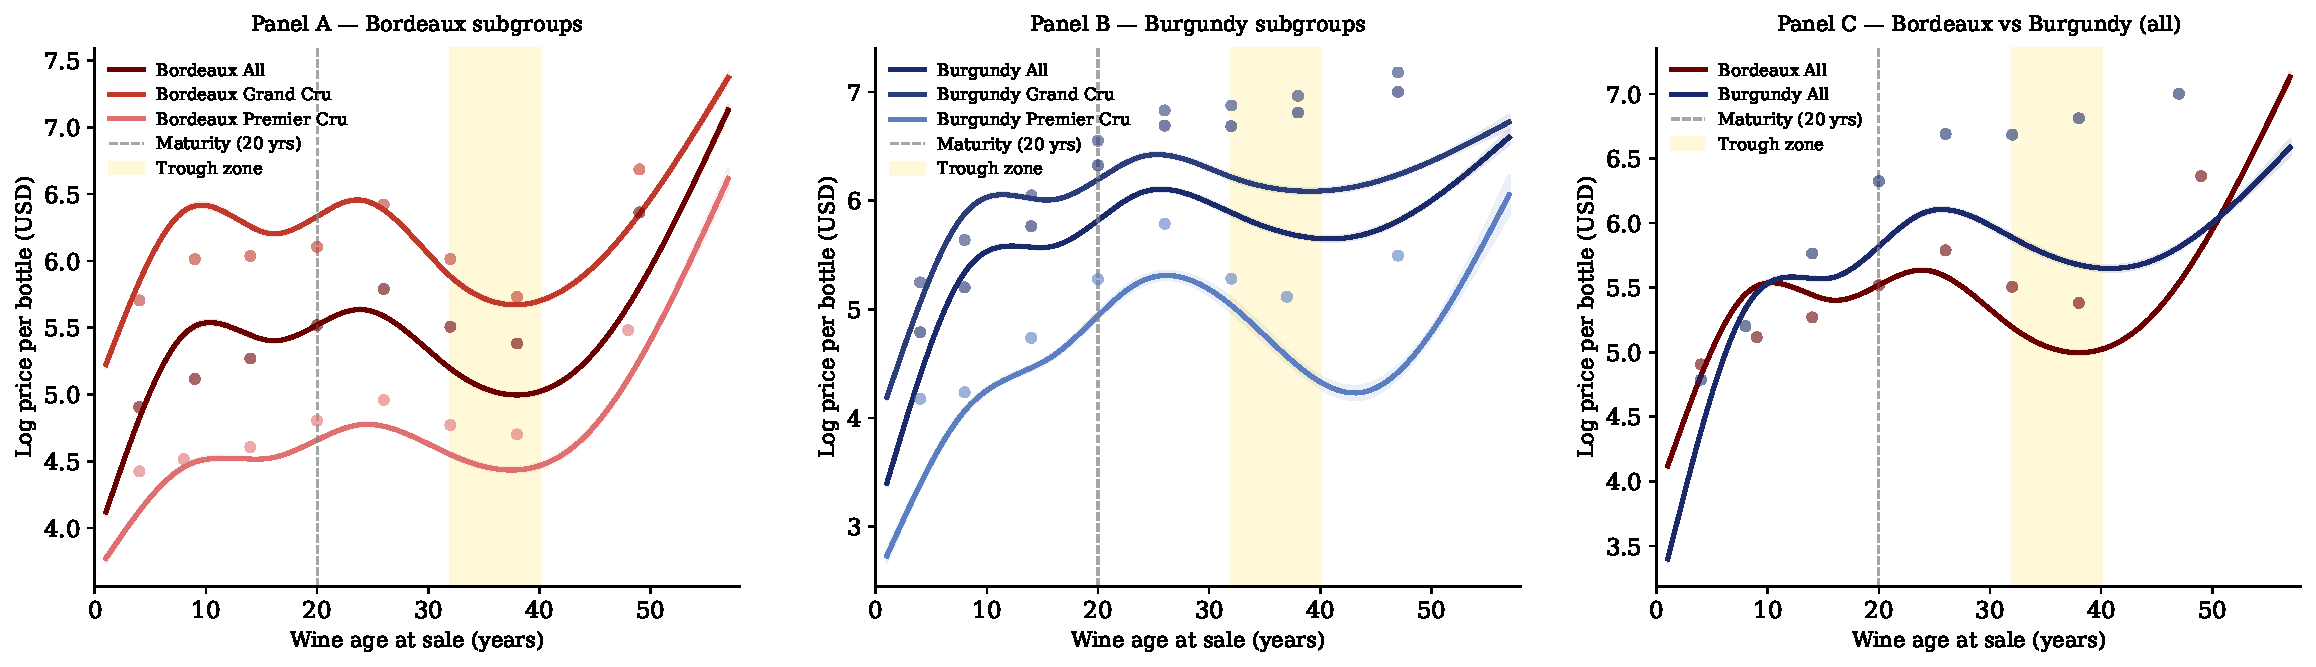
\includegraphics[width=\textwidth]{figures/fig_spline_comparison.pdf}
  \caption{Price-age profiles estimated by natural cubic spline (knots at
    $a^* \in \{0.4, 0.8, 1.2, 1.6, 2.2\}$) with 95\,\% confidence bands (shaded).
    \textit{Panel A}: Bordeaux subgroups (All, Grand Cru, Premier Cru).
    \textit{Panel B}: Burgundy subgroups (All, Grand Cru, Premier Cru).
    \textit{Panel C}: Bordeaux All vs.\ Burgundy All.
    Dots are binned medians (bin width: 0.30 normalised-age units).
    The dashed vertical line marks the maturity threshold (20 years);
    the shaded yellow band indicates the trough zone (approximately 32--40 years,
    $a^* \in [1.6, 2.0)$).
    $x$-axis is calendar age in years (normalised age $\times$ 20-year cap).
    Sample: 1996--2015 auction lots.}
  \label{fig:spline}
\end{figure}

\subsection{Statistical significance of the dip}

Tables~\ref{tab:segment_dip_bordeaux} and~\ref{tab:segment_dip_burgundy} report the segment
dummy regressions for Bordeaux and Burgundy groups respectively, each in four specifications:
(1) baseline, (2) vintage year fixed effects, (3) producer fixed effects, and (4) both fixed
effects simultaneously.

For Bordeaux Grand Cru, the trough segment is substantially below the peak segment across all
four specifications, and the Trough~$-$~Peak contrast is significant at the 0.1\,\% level.
Bordeaux Premier Cru likewise shows a statistically significant dip. The magnitudes are
broadly stable when adding vintage or producer fixed effects, confirming that the trough is not
a cohort quality effect or a producer compositional artifact.

Burgundy Grand Cru shows the opposite: the trough segment is \textit{above} the peak in all
specifications, consistent with a monotonically rising profile and the absence of
consumer-demand exit.

\begin{table}[htbp]
\centering
\caption{Price-age segment regression: Bordeaux groups}
\label{tab:segment_dip_bordeaux}
\resizebox{\textwidth}{!}{%
\begin{tabular}{lcccccccccccc}
\toprule
 & \multicolumn{4}{c}{Bordeaux All} & \multicolumn{4}{c}{Bordeaux Grand Cru} & \multicolumn{4}{c}{Bordeaux Premier Cru} \\
\cmidrule(lr){2-5}\cmidrule(lr){6-9}\cmidrule(lr){10-13}
Segment (base: young) & (1) & (2) & (3) & (4) & (1) & (2) & (3) & (4) & (1) & (2) & (3) & (4) \\
\midrule
\textit{Approach} & $0.179^{***}$ & $0.603^{***}$ & $0.179^{***}$ & $0.603^{***}$ & $0.058^{***}$ & $0.631^{***}$ & $0.058^{***}$ & $0.631^{***}$ & $0.117^{***}$ & $0.330^{***}$ & $0.117^{***}$ & $0.330^{***}$ \\
  & (0.005) & (0.005) & (0.005) & (0.005) & (0.006) & (0.006) & (0.006) & (0.006) & (0.005) & (0.005) & (0.005) & (0.005) \\
\textit{Peak} & $0.467^{***}$ & $1.385^{***}$ & $0.467^{***}$ & $1.385^{***}$ & $0.276^{***}$ & $1.433^{***}$ & $0.276^{***}$ & $1.433^{***}$ & $0.371^{***}$ & $0.860^{***}$ & $0.371^{***}$ & $0.860^{***}$ \\
  & (0.005) & (0.007) & (0.005) & (0.007) & (0.006) & (0.008) & (0.006) & (0.008) & (0.006) & (0.008) & (0.006) & (0.008) \\
\textit{Trough} & $0.163^{***}$ & $1.903^{***}$ & $0.163^{***}$ & $1.903^{***}$ & $-0.214^{***}$ & $1.977^{***}$ & $-0.214^{***}$ & $1.977^{***}$ & $0.228^{***}$ & $1.211^{***}$ & $0.228^{***}$ & $1.211^{***}$ \\
  & (0.008) & (0.012) & (0.008) & (0.012) & (0.010) & (0.013) & (0.010) & (0.013) & (0.011) & (0.014) & (0.011) & (0.014) \\
\textit{Antique} & $1.076^{***}$ & $2.597^{***}$ & $1.076^{***}$ & $2.597^{***}$ & $0.602^{***}$ & $2.735^{***}$ & $0.602^{***}$ & $2.735^{***}$ & $0.994^{***}$ & $1.673^{***}$ & $0.994^{***}$ & $1.673^{***}$ \\
  & (0.008) & (0.016) & (0.008) & (0.016) & (0.009) & (0.018) & (0.009) & (0.018) & (0.013) & (0.021) & (0.013) & (0.021) \\
\midrule
\textbf{Trough $-$ Peak} & $-0.304^{***}$ & $0.518$ & $-0.304^{***}$ & $0.518$ & $-0.490^{***}$ & $0.544$ & $-0.490^{***}$ & $0.544$ & $-0.143^{***}$ & $0.351$ & $-0.143^{***}$ & $0.351$ \\
  & (-26.2\%) & (+67.9\%) & (-26.2\%) & (+67.9\%) & (-38.8\%) & (+72.2\%) & (-38.8\%) & (+72.2\%) & (-13.3\%) & (+42.1\%) & (-13.3\%) & (+42.1\%) \\
\midrule
$R^2$ & 0.054 & 0.205 & 0.054 & 0.205 & 0.036 & 0.364 & 0.036 & 0.364 & 0.055 & 0.228 & 0.055 & 0.228 \\
$N$ & 436,413 & 436,413 & 436,413 & 436,413 & 215,036 & 215,036 & 215,036 & 215,036 & 221,377 & 221,377 & 221,377 & 221,377 \\
Vintage FE & No & Yes & No & Yes & No & Yes & No & Yes & No & Yes & No & Yes \\
Producer FE & No & No & Yes & Yes & No & No & Yes & Yes & No & No & Yes & Yes \\
\bottomrule
\end{tabular}
}
\par\vspace{4pt}
{\footnotesize\textit{Notes:} OLS, dependent variable log price per bottle (USD). Robust (HC1) standard errors in parentheses. Segments: \textit{young} = $a^* \in [0, 0.6)$; \textit{approach} $\in [0.6, 1.0)$; \textit{peak} $\in [1.0, 1.6)$; \textit{trough} $\in [1.6, 2.0)$; \textit{antique} $\in [2.0, 3.0]$. ``Trough $-$ Peak'' reports the direct contrast with one-sided $p$-value (trough $<$ peak). (1) Baseline. (2) Vintage FE. (3) Producer FE. (4) Both FE. $^{***}p<0.001$, $^{**}p<0.01$, $^{*}p<0.05$.}
\end{table}


\begin{table}[htbp]
\centering
\caption{Price-age segment regression: Burgundy groups}
\label{tab:segment_dip_burgundy}
\resizebox{\textwidth}{!}{%
\begin{tabular}{lcccccccccccc}
\toprule
 & \multicolumn{4}{c}{Burgundy All} & \multicolumn{4}{c}{Burgundy Grand Cru} & \multicolumn{4}{c}{Burgundy Premier Cru} \\
\cmidrule(lr){2-5}\cmidrule(lr){6-9}\cmidrule(lr){10-13}
Segment (base: young) & (1) & (2) & (3) & (4) & (1) & (2) & (3) & (4) & (1) & (2) & (3) & (4) \\
\midrule
\textit{Approach} & $0.625^{***}$ & $0.964^{***}$ & $0.625^{***}$ & $0.964^{***}$ & $0.477^{***}$ & $0.832^{***}$ & $0.477^{***}$ & $0.832^{***}$ & $0.621^{***}$ & $0.922^{***}$ & $0.621^{***}$ & $0.922^{***}$ \\
  & (0.006) & (0.006) & (0.006) & (0.006) & (0.007) & (0.007) & (0.007) & (0.007) & (0.010) & (0.010) & (0.010) & (0.010) \\
\textit{Peak} & $1.314^{***}$ & $1.951^{***}$ & $1.314^{***}$ & $1.951^{***}$ & $1.046^{***}$ & $1.699^{***}$ & $1.046^{***}$ & $1.699^{***}$ & $1.407^{***}$ & $2.174^{***}$ & $1.407^{***}$ & $2.174^{***}$ \\
  & (0.008) & (0.012) & (0.008) & (0.012) & (0.009) & (0.012) & (0.009) & (0.012) & (0.019) & (0.024) & (0.019) & (0.024) \\
\textit{Trough} & $1.505^{***}$ & $2.773^{***}$ & $1.505^{***}$ & $2.773^{***}$ & $1.271^{***}$ & $2.567^{***}$ & $1.271^{***}$ & $2.567^{***}$ & $1.154^{***}$ & $2.911^{***}$ & $1.154^{***}$ & $2.911^{***}$ \\
  & (0.017) & (0.029) & (0.017) & (0.029) & (0.018) & (0.029) & (0.018) & (0.029) & (0.045) & (0.075) & (0.045) & (0.075) \\
\textit{Antique} & $1.726^{***}$ & $3.438^{***}$ & $1.726^{***}$ & $3.438^{***}$ & $1.451^{***}$ & $3.215^{***}$ & $1.451^{***}$ & $3.215^{***}$ & $1.201^{***}$ & $3.654^{***}$ & $1.201^{***}$ & $3.654^{***}$ \\
  & (0.013) & (0.038) & (0.013) & (0.038) & (0.013) & (0.038) & (0.013) & (0.038) & (0.030) & (0.092) & (0.030) & (0.092) \\
\midrule
\textbf{Trough $-$ Peak} & $0.191$ & $0.821$ & $0.191$ & $0.821$ & $0.225$ & $0.869$ & $0.225$ & $0.869$ & $-0.253^{***}$ & $0.737$ & $-0.253^{***}$ & $0.737$ \\
  & (+21.0\%) & (+127.4\%) & (+21.0\%) & (+127.4\%) & (+25.3\%) & (+138.3\%) & (+25.3\%) & (+138.3\%) & (-22.4\%) & (+109.0\%) & (-22.4\%) & (+109.0\%) \\
\midrule
$R^2$ & 0.142 & 0.205 & 0.142 & 0.205 & 0.118 & 0.195 & 0.118 & 0.195 & 0.150 & 0.239 & 0.150 & 0.239 \\
$N$ & 308,648 & 308,648 & 308,648 & 308,648 & 221,512 & 221,512 & 221,512 & 221,512 & 87,136 & 87,136 & 87,136 & 87,136 \\
Vintage FE & No & Yes & No & Yes & No & Yes & No & Yes & No & Yes & No & Yes \\
Producer FE & No & No & Yes & Yes & No & No & Yes & Yes & No & No & Yes & Yes \\
\bottomrule
\end{tabular}
}
\par\vspace{4pt}
{\footnotesize\textit{Notes:} OLS, dependent variable log price per bottle (USD). Robust (HC1) standard errors in parentheses. Segments: \textit{young} = $a^* \in [0, 0.6)$; \textit{approach} $\in [0.6, 1.0)$; \textit{peak} $\in [1.0, 1.6)$; \textit{trough} $\in [1.6, 2.0)$; \textit{antique} $\in [2.0, 3.0]$. ``Trough $-$ Peak'' reports the direct contrast with one-sided $p$-value (trough $<$ peak). (1) Baseline. (2) Vintage FE. (3) Producer FE. (4) Both FE. $^{***}p<0.001$, $^{**}p<0.01$, $^{*}p<0.05$.}
\end{table}


\subsection{Piecewise linear robustness: negative trough slopes}

Table~\ref{tab:piecewise_slopes} reports the piecewise linear specification~\eqref{eq:piecewise}.
The trough slope $\beta_1 + \beta_2$ is negative for both Bordeaux groups (Bordeaux All:
$-0.020$; Bordeaux Grand Cru: $-0.261$), confirming that prices \emph{fall} with age in the
post-maturity period for Bordeaux wines. The deeper slope for Bordeaux Grand Cru reflects the
higher consumption valuations at peak maturity for the premier châteaux, which create a larger
correction when consumption buyers exit.

In contrast, the trough slope is positive and large for both Burgundy groups (Burgundy Grand
Cru: $+0.569$; Burgundy Premier Cru: $+0.403$), indicating that prices continue to rise
monotonically after maturity.

\begin{table}[htbp]
\centering
\caption{Piecewise linear price-age slopes by wine group}
\label{tab:piecewise_slopes}
\small
\begin{threeparttable}
\begin{tabular}{lcccccc}
\toprule
 & \multicolumn{1}{c}{Bx All} & \multicolumn{1}{c}{Bx GC} & \multicolumn{1}{c}{Bx PC} & \multicolumn{1}{c}{Bu All} & \multicolumn{1}{c}{Bu GC} & \multicolumn{1}{c}{Bu PC} \\
\midrule
$\beta_1$ (pre-maturity slope) & $0.6286^{***}$ & $0.4226^{***}$ & $0.4321^{***}$ & $1.6722^{***}$ & $1.3449^{***}$ & $1.5511^{***}$ \\
  & (0.0077) & (0.0101) & (0.0084) & (0.0099) & (0.0111) & (0.0172) \\
$\beta_2$ (change at maturity) & $-0.6487^{***}$ & $-0.6831^{***}$ & $-0.3265^{***}$ & $-1.0577^{***}$ & $-0.7757^{***}$ & $-1.1479^{***}$ \\
  & (0.0141) & (0.0175) & (0.0174) & (0.0226) & (0.0238) & (0.0498) \\
$\beta_3$ (change at antique) & $1.7404^{***}$ & $1.7145^{***}$ & $1.5738^{***}$ & $-0.5092^{***}$ & $-0.5041^{***}$ & $-0.5567^{***}$ \\
  & (0.0238) & (0.0266) & (0.0392) & (0.0449) & (0.0452) & (0.1257) \\
\midrule
\textbf{Trough slope} $\beta_1+\beta_2$ & $-0.0201^{**}$ & $-0.2606^{***}$ & $0.1056^{***}$ & $0.6145^{***}$ & $0.5692^{***}$ & $0.4032^{***}$ \\
  & (0.0086) & (0.0101) & (0.0116) & (0.0160) & (0.0163) & (0.0405) \\
\midrule
$R^2$ & 0.063 & 0.042 & 0.064 & 0.156 & 0.128 & 0.150 \\
$N$ & 436,413 & 215,036 & 221,377 & 308,648 & 221,512 & 87,136 \\
\bottomrule
\end{tabular}
\begin{tablenotes}
\footnotesize
\item Notes: OLS piecewise linear regression. Dependent variable: log price per bottle (USD).
  Model: $\log p = \alpha + \beta_1 a^* + \beta_2 (a^*-1)_+ + \beta_3 (a^*-2)_+ + \varepsilon$
  where $(x)_+ = \max(0,x)$.
  The slope in the trough zone ($a^* \in [1,2)$) is $\beta_1+\beta_2$; negative values indicate
  a declining price-age profile in the post-maturity period.
  Robust (HC1) standard errors in parentheses.
  $^{***}p<0.01$, $^{**}p<0.05$, $^{*}p<0.10$.
\end{tablenotes}
\end{threeparttable}
\end{table}


\subsection{Mechanism: collector composition and the price floor}

Table~\ref{tab:summary_stats} documents the key cross-sectional difference that rationalises
the contrasting profiles. Among young lots ($a^* < 0.4$, i.e., wines under 8 years old),
Burgundy Grand Cru commands the highest share of transactions above \$200 per bottle,
followed by Bordeaux Grand Cru and Bordeaux All, with Burgundy Premier Cru at the bottom.
The high entry price of Burgundy Grand Cru screens out consumption buyers from the outset:
a bidder who intends to drink the wine must be willing to pay collector-level prices even when
the wine is young. There is no consumption demand segment to exit at peak maturity, hence no
downward price pressure in the trough zone.

\begin{table}[htbp]
\centering
\caption{Sample summary statistics by wine group}
\label{tab:summary_stats}
\small
\begin{threeparttable}
\begin{tabular}{lrrrrrrr}
\toprule
 & & \multicolumn{2}{c}{Share} & \multicolumn{3}{c}{Median price (\$/bottle)} & \\
\cmidrule(lr){3-4}\cmidrule(lr){5-7}
Group & $N$ & Post-mat. & Coll.$^{a}$ & Young & At peak & Antique & Med. age \\
 & & (\%) & (\%) & & & & (yrs) \\
\midrule
Bordeaux All & 436,413 & 35.2 & 39.0 & \$140 & \$237 & \$532 & 16 \\
Bordeaux Grand Cru & 215,036 & 39.8 & 68.5 & \$336 & \$431 & \$748 & 17 \\
Bordeaux Premier Cru & 221,377 & 30.6 & 19.1 & \$85 & \$118 & \$220 & 14 \\
\midrule
Burgundy All & 308,648 & 18.5 & 36.8 & \$133 & \$504 & \$1,074 & 11 \\
Burgundy Grand Cru & 221,512 & 21.5 & 51.5 & \$213 & \$635 & \$1,278 & 11 \\
Burgundy Premier Cru & 87,136 & 10.9 & 11.2 & \$65 & \$170 & \$231 & 9 \\
\bottomrule
\end{tabular}
\begin{tablenotes}
\footnotesize
\item Notes: ``Young'' = age\textsubscript{norm} $<$ 0.4 ($<$ 8 years).
  ``At peak'' = age\textsubscript{norm} $\in$ [0.9, 1.1] (18--22 years).
  ``Antique'' = age\textsubscript{norm} $>$ 2.0 ($>$ 40 years).
  $^{a}$ Share of young lots priced $>$ \$200/bottle.
  Maturity cap: 20 years. Sample period: 1996--2015.
\end{tablenotes}
\end{threeparttable}
\end{table}


\subsection{Heterogeneity by wine-specific maturity}
\label{sec:results:heterogeneity}

\noindent\textit{[To be completed. Key result to document: the dip is not an artifact of
the maturity normalisation. Within the Bordeaux Grand Cru group, wines with shorter
maturity windows (say, $\tau_i < 18$ years) exhibit a shallower trough than wines with
longer maturity windows ($\tau_i \geq 22$ years), consistent with Proposition~\ref{prop:compstat}(iii)
--- a sharper consumption peak deepens the trough.
Show Table~X stratifying segment regression by tercile of $\tau_i$.]}

\subsection{Price-age medians: raw evidence}
\label{sec:results:medians}

Appendix~\ref{app:medians} reports binned log price medians by normalised age bin (width 0.2)
for all six groups. The raw medians confirm the spline shape without any smoothing assumption.

% ============================================================
%  Section 3 — A Model of Collector and Consumer Demand
% ============================================================

\section{A Model of Collector and Consumer Demand}
\label{sec:model}

We develop a parsimonious auction model with heterogeneous buyers to
rationalize the non-monotone price-age profile documented in
Section~\ref{sec:results}.  The model builds on the two-type framework
of \citet{lovo2018}, adapted to the distinctive feature of wine:
a biological maturity date after which consumption value declines.

%% ── 3.1  Environment ────────────────────────────────────────────

\subsection{Environment}
\label{sec:model:env}

Consider a single bottle of wine with vintage-specific maturity date
$\tau > 0$ (years since vintage).  The bottle reaches auction at age
$a \geq 0$; we work throughout with \emph{normalised age}
$a^{*} \equiv a / \tau$, so that $a^{*} = 1$ corresponds to peak
maturity.

In each auction, $n \geq 2$ risk-neutral potential bidders compete in a
second-price sealed-bid (Vickrey) mechanism.  Each bidder is
independently drawn as one of two types:
\begin{itemize}
  \item \textbf{Consumption buyers} (type~$c$), with probability
        $\lambda(a^{*})$, value wine for drinking.
  \item \textbf{Collector buyers} (type~$k$), with probability
        $1 - \lambda(a^{*})$, value wine for holding, prestige, or
        future resale.
\end{itemize}
Valuations are independent private values: each bidder knows her own
type and valuation but not those of others.  Truthful bidding is
weakly dominant, so the auction price equals the second-highest
valuation among the~$n$ bidders.

%% ── 3.2  Primitives ─────────────────────────────────────────────

\subsection{Primitives}
\label{sec:model:primitives}

\begin{assumption}[Consumption Valuation]
\label{as:vc}
The consumption-buyer valuation is
\begin{equation}
  v_{c}(a^{*})
  = \alpha_{c}\, h(a^{*}),
  \qquad
  h(a^{*})
  = (a^{*})^{\gamma}\, e^{\,\gamma(1 - a^{*})},
  \quad \gamma > 0,
  \label{eq:vc}
\end{equation}
where $\alpha_{c} > 0$ is the maximum consumption value (attained at
$a^{*} = 1$).  The quality function~$h$ satisfies $h(0) = 0$,
$h(1) = 1$, is strictly increasing on $[0,1]$, strictly decreasing
on $(1,\infty)$, and $h(a^{*}) \to 0$ as $a^{*} \to \infty$.  The
parameter~$\gamma$ controls peakedness: higher~$\gamma$ implies a
sharper peak at maturity and faster post-maturity decay.
\end{assumption}

\begin{assumption}[Collector Valuation]
\label{as:vk}
The collector-buyer valuation is
\begin{equation}
  v_{k}(a^{*})
  = \bar{v}_{k} + \alpha_{k}\, a^{*},
  \qquad
  \bar{v}_{k} > 0,
  \quad \alpha_{k} \geq 0.
  \label{eq:vk}
\end{equation}
The parameter~$\bar{v}_{k}$ is the baseline collector value---the
``price floor'' reflecting scarcity, prestige, and storage of fine
wine---and $\alpha_{k}$ captures the incremental age premium.
\end{assumption}

\begin{assumption}[Buyer Composition]
\label{as:lambda}
The probability that a given bidder is type~$c$ is
\begin{equation}
  \lambda(a^{*})
  = \begin{cases}
      \bar{\lambda}
        & \text{if } a^{*} \leq 1, \\[4pt]
      \bar{\lambda}\, e^{-\delta(a^{*} - 1)}
        & \text{if } a^{*} > 1,
    \end{cases}
  \qquad
  \bar{\lambda} \in (0,1),
  \quad \delta > 0.
  \label{eq:lambda}
\end{equation}
Consumption buyers participate at a constant rate~$\bar{\lambda}$
before maturity and exit at rate~$\delta$ afterward, reflecting
declining interest in a wine that is past its drinking peak.
\end{assumption}

\noindent
The model has six parameters:
$(\alpha_{c},\, \bar{v}_{k},\, \alpha_{k},\, \gamma,\, \delta,\,
\bar{\lambda})$.  We suppress dependence on~$n$ (number of bidders)
in the notation; all results hold for any fixed $n \geq 2$.

%% ── 3.3  Equilibrium Price ──────────────────────────────────────

\subsection{Equilibrium Price}
\label{sec:model:equil}

Under truthful bidding, the auction price equals the second-highest
valuation.  Because each bidder's valuation is deterministic
conditional on type, the $n$ bids are i.i.d.\ draws from the
two-point distribution
$\{v_{c}(a^{*}),\, v_{k}(a^{*})\}$ with probabilities
$\{\lambda(a^{*}),\, 1 - \lambda(a^{*})\}$.

\medskip

\noindent\textbf{Definition (Equilibrium price).}
The expected auction price at normalised age~$a^{*}$ is
\begin{equation}
  P(a^{*})
  = \mathbb{E}\!\left[\,V_{(n-1:n)} \,\big|\, a^{*}\,\right],
  \label{eq:price}
\end{equation}
where $V_{(n-1:n)}$ denotes the second-order statistic of the~$n$
valuations.

\medskip

Write $\lambda = \lambda(a^{*})$, $v_{c} = v_{c}(a^{*})$,
$v_{k} = v_{k}(a^{*})$.  When $v_{c} \geq v_{k}$ (which holds near
maturity under Assumption~\ref{as:vc}--\ref{as:vk}), the
second-highest bid equals~$v_{c}$ if and only if at least two of the
$n$~bidders are type~$c$.  Letting
$q_{0} = (1-\lambda)^{n}$ and
$q_{1} = n\,\lambda\,(1-\lambda)^{n-1}$:
\begin{equation}
  P(a^{*})
  = v_{c}\!\left(1 - q_{0} - q_{1}\right)
  + v_{k}\!\left(q_{0} + q_{1}\right)
  \qquad \text{when } v_{c} \geq v_{k}.
  \label{eq:price_vc_dom}
\end{equation}
When $v_{k} > v_{c}$ (deep post-maturity), the symmetric expression
holds with $r_{0} = \lambda^{n}$ and
$r_{1} = n\,(1-\lambda)\,\lambda^{n-1}$:
\begin{equation}
  P(a^{*})
  = v_{k}\!\left(1 - r_{0} - r_{1}\right)
  + v_{c}\!\left(r_{0} + r_{1}\right)
  \qquad \text{when } v_{k} > v_{c}.
  \label{eq:price_vk_dom}
\end{equation}
In either case, $P(a^{*})$ is a weighted average of the two
valuations, with the weight on the higher valuation equal to the
probability that the second-order statistic equals that value.

%% ── 3.4  Main Results ───────────────────────────────────────────

\subsection{Main Results}
\label{sec:model:results}

\begin{proposition}[Non-Monotone Price-Age Profile]
\label{prop:nonmono}
Suppose\, $\alpha_{c} > \bar{v}_{k} + \alpha_{k}$
(consumption value at maturity exceeds collector value at maturity),
$\gamma > 0$, $\delta > 0$, and $n \geq 2$.  Then there exist
$a^{*}_{\mathrm{peak}}$ and $a^{*}_{\mathrm{trough}}$ with
$1 \leq a^{*}_{\mathrm{peak}} < a^{*}_{\mathrm{trough}}$ such that:
\begin{enumerate}
  \item[\emph{(i)}]
    $P(a^{*})$ is strictly increasing on
    $[0,\, a^{*}_{\mathrm{peak}}]$.
  \item[\emph{(ii)}]
    $P(a^{*})$ is strictly decreasing on
    $[a^{*}_{\mathrm{peak}},\, a^{*}_{\mathrm{trough}}]$.
  \item[\emph{(iii)}]
    $P(a^{*})$ is eventually strictly increasing for~$a^{*}$
    sufficiently large.
\end{enumerate}
\end{proposition}

\begin{proof}[Proof sketch]
Three forces shape the price path.
\emph{Pre-maturity} ($a^{*} \leq 1$): both $v_{c}$ and~$v_{k}$ are
increasing and $\lambda$ is constant, so $P$ is increasing.
\emph{Post-maturity transition} ($a^{*}$ slightly above~$1$):
$v_{c}$ decays at rate~$\gamma$ (Assumption~\ref{as:vc}) and
$\lambda$ decays at rate~$\delta$ (Assumption~\ref{as:lambda}).
Both effects reduce the probability that the second-highest bidder
is type~$c$, and since $v_{c} > v_{k}$ in a neighbourhood of
$a^{*} = 1$, the price falls---the \emph{composition effect}
dominates.
\emph{Recovery} ($a^{*} \to \infty$): $\lambda \to 0$ and
$v_{c} \to 0$, so the auction is populated entirely by collectors.
The price converges to~$v_{k}(a^{*})$, which is increasing.
The trough is the age at which the declining composition effect is
exactly offset by the rising collector premium.
A formal proof is in Appendix~\ref{app:proofs}.
\end{proof}

\medskip

The next result explains why the trough is absent for Burgundy Grand
Cru.

\begin{proposition}[Trough Disappearance]
\label{prop:notrough}
Define the collector-dominance ratio
$\rho \equiv \bar{v}_{k} / \alpha_{c}$.
There exists a threshold~$\rho^{*} \in (0,1)$ such that if
$\rho > \rho^{*}$, then $P(a^{*})$ is weakly increasing for all
$a^{*} \geq 0$.
\end{proposition}

\begin{proof}[Proof sketch]
When $\rho \geq 1$, we have $\bar{v}_{k} \geq \alpha_{c}$, so
$v_{k}(a^{*}) \geq \bar{v}_{k} \geq \alpha_{c} \geq v_{c}(a^{*})$
for all~$a^{*}$.  Collectors dominate every auction, and the price
tracks the increasing function~$v_{k}$.
For $\rho < 1$ but $\rho > \rho^{*}$, there exists a narrow interval
near $a^{*} = 1$ where $v_{c}$ exceeds~$v_{k}$, but the interval is
too short and the consumption share~$\bar{\lambda}$ too small for
the composition effect to generate a net price decline.
The threshold~$\rho^{*}$ depends on $(\gamma, \delta, \bar{\lambda},
\alpha_{k}, n)$; a formal characterisation is in
Appendix~\ref{app:proofs}.
\end{proof}

\noindent
The ratio~$\rho$ has a direct empirical counterpart: the share of
young auction lots (normalised age below~0.4) whose per-bottle price
exceeds~\$200.  This share proxies for the intensity of collector
demand at early ages.  Table~\ref{tab:rho_mapping} summarises the
cross-sectional mapping.

\begin{table}[htbp]
\centering
\caption{Collector-Dominance Ratio and Trough Presence}
\label{tab:rho_mapping}
\begin{tabular}{lccc}
\toprule
Category & Young lots $>$ \$200 & Implied $\rho$ & Trough \\
\midrule
Burgundy Grand Cru     & 51.5\% & High ($> \rho^{*}$) & Absent \\
Bordeaux Crus Class\'es & 39.0\% & Moderate ($< \rho^{*}$) & $-26.2\%$ \\
Burgundy Premier Cru   & 11.2\% & Low ($\ll \rho^{*}$) & $-22.4\%$ \\
\bottomrule
\end{tabular}
\end{table}

\begin{proposition}[Comparative Statics on Trough Depth]
\label{prop:compstat}
For a wine category with $\rho < \rho^{*}$, define the trough depth
$\Delta \equiv P(a^{*}_{\mathrm{peak}}) -
P(a^{*}_{\mathrm{trough}})$.  Then:
\begin{enumerate}
  \item[\emph{(i)}]
    $\partial \Delta / \partial \bar{\lambda} > 0$: a higher
    consumption-buyer share deepens the trough.
  \item[\emph{(ii)}]
    $\partial \Delta / \partial \bar{v}_{k} < 0$: a higher collector
    floor compresses the trough.
  \item[\emph{(iii)}]
    $\partial \Delta / \partial \gamma > 0$: a sharper consumption
    peak deepens the trough.
  \item[\emph{(iv)}]
    $\partial \Delta / \partial \delta > 0$: faster consumption-buyer
    exit deepens the trough.
\end{enumerate}
\end{proposition}

\begin{proof}[Proof sketch]
Part~\emph{(i)}: higher~$\bar{\lambda}$ increases competition among
consumption buyers near maturity, raising
$P(a^{*}_{\mathrm{peak}})$.  After maturity, the same buyers exit,
so $P(a^{*}_{\mathrm{trough}})$ falls---the gap widens.
Part~\emph{(ii)}: higher~$\bar{v}_{k}$ raises the price floor set
by collectors, truncating the price decline at the trough.
Parts~\emph{(iii)}--\emph{(iv)} accelerate the post-maturity
collapse of consumption demand, steepening the transition from peak
to trough.
Formal proofs are in Appendix~\ref{app:proofs}.
\end{proof}

%% ── 3.5  Empirical Predictions ──────────────────────────────────

\subsection{Empirical Predictions}
\label{sec:model:predictions}

The model yields four testable implications that we take to the data
in Sections~\ref{sec:empirics}--\ref{sec:results}.

\medskip

\noindent\textbf{Prediction~1} (Non-monotone profile).
For wine categories in which consumption buyers constitute a
substantial share of bidders ($\rho < \rho^{*}$), the log price-age
profile should rise pre-maturity, fall post-maturity, and recover at
antique ages.

\medskip

\noindent\textbf{Prediction~2} (Trough disappearance).
Wine categories where the collector-dominance ratio is sufficiently
high---observable as a high share of young lots priced above \$200
per bottle---should exhibit a monotonically increasing price-age
profile with no post-maturity trough.

\medskip

\noindent\textbf{Prediction~3} (Monotone pre-maturity rise).
All categories should show rising prices pre-maturity, because both
consumption and collector valuations are increasing before $a^{*}=1$.

\medskip

\noindent\textbf{Prediction~4} (Cross-sectional trough depth).
Across categories that exhibit a trough, its depth should be
increasing in the consumption-buyer share and decreasing in the
collector-value floor.

%% ── 3.6  Discussion ─────────────────────────────────────────────

\subsection{Discussion}
\label{sec:model:discussion}

\paragraph{Relationship to \citet{lovo2018}.}
Our model shares the two-type buyer structure with the art-market
model of \citet{lovo2018}, but differs in three key respects.
First, wine has a finite consumption life governed by the maturity
date~$\tau$, which generates the single-peaked consumption valuation
$v_{c}(a^{*})$ central to the non-monotone price profile.
Art has no biological expiry, so the consumption-type valuation in
\citet{lovo2018} is constant.
Second, the maturity date varies across wines and is (imperfectly)
observable via expert tasting notes, providing cross-sectional
variation in~$a^{*}$ that identifies the model.
Third, we adopt a static auction mechanism appropriate for the
institutional setting, rather than the dynamic search-and-matching
framework of \citet{lovo2018}.

\paragraph{Why arbitrageurs do not eliminate the trough.}
If collectors could costlessly buy at the trough and resell at
antique ages, forward-looking bidding would compress the price dip.
The persistence of the trough in the data points to significant
frictions: storage costs (approximately 1--2\,\% of value per year
for temperature-controlled storage), authentication risk (provenance
uncertainty rises with the number of transactions), and thin markets
(low trading frequency for post-maturity wines reduces liquidity).

\paragraph{Endogenous supply.}
The baseline model takes supply as given.  If sellers anticipate
lower prices in the trough zone, they may delay consignment,
reducing supply and partially offsetting the price decline.  The fact
that the trough persists suggests that seller delay, while plausible,
does not fully eliminate the composition-driven dip.

\paragraph{Structural estimation.}
The six model parameters
$(\alpha_{c}, \bar{v}_{k}, \alpha_{k}, \gamma, \delta,
\bar{\lambda})$ can be estimated by matching the observed price-age
profiles across wine categories using minimum distance, with 7
moment conditions (8 age bins, young as baseline) and the full
HC1-robust covariance matrix as optimal weight.
Appendix~\ref{app:structural} describes the estimation procedure and
will report these estimates for all three grand cru categories, together
with a $J$-test of overidentification and parametric bootstrap
confidence sets.
\textit{[Placeholder: structural estimation results to be completed.
The estimated $\rho = \bar{v}_{k}/\alpha_{c}$ is expected to exceed
unity for Burgundy Grand Cru, confirming Proposition~\ref{prop:notrough}.
]}          % ← Model section: edit model.tex directly
% ============================================================
%  Section 6 — Conclusion  (placeholder)
% ============================================================

\section{Conclusion}
\label{sec:conclusion}

\noindent\textit{[To be completed. Planned structure:]}

\noindent\textit{\textbf{Summary paragraph.} Restate the main finding: the price-age profile of
top French wines is non-monotone; the trough zone (32--40 years post-vintage) is a structural
feature of demand composition, not noise. Burgundy Grand Cru avoids the trough because its
entry price screens out consumption buyers.}

\noindent\textit{\textbf{Contribution paragraph.} We provide (i) direct evidence on how buyer
heterogeneity shapes asset prices at a key life-cycle transition; (ii) a clean identification
strategy exploiting wine-specific maturity dates; (iii) a tractable structural model that
rationalises the cross-sectional patterns and yields testable comparative statics.}

\noindent\textit{\textbf{Broader implications paragraph.} Results speak to the general class
of storable durable goods with maturity (whisky, aged spirits, vintage cars, art with condition
degradation). The mechanism — exit of consumption buyers at a quality threshold — should appear
in any market with two-type demand and finite consumption value.}

\noindent\textit{\textbf{Limitations and future work.} Endogenous supply (seller timing),
dynamic buyer strategies, and the role of financial intermediaries (wine funds, storage
platforms) are left to future work.}


% ── Bibliography ─────────────────────────────────────────────────────────────
\newpage
\bibliographystyle{aer}
\bibliography{references}

% ── Appendix ─────────────────────────────────────────────────────────────────
\newpage
% ============================================================
%  Online Appendix
% ============================================================

\appendix

\section{Full Sample Statistics}
\label{app:full_sample}

Table~\ref{tab:full_sample} reports lot counts and median prices for the full auction
sample broken down by region and wine type.

\begin{table}[htbp]
\centering
\caption{Full sample summary statistics (all lots, by region and type)}
\label{tab:full_sample}
\small
\begin{threeparttable}
\begin{tabular}{llrrrrr}
\toprule
Region & Type & $N$ & Med. price & Med. age & Pre-mat. & Post-mat. \\
 & & & (\$/bottle) & (yrs) & (\%) & (\%) \\
\midrule
Bordeaux & red & 575,837 & \$181 & 14 & 65.8 & 31.9 \\
Bordeaux & white & 39,241 & \$118 & 15 & 61.7 & 35.7 \\
Burgundy & red & 224,457 & \$313 & 12 & 75.5 & 22.5 \\
Burgundy & white & 103,914 & \$136 & 8 & 90.7 & 8.1 \\
Rhone & red & 91,300 & \$115 & 9 & 84.7 & 13.5 \\
Rhone & white & 14,150 & \$110 & 6 & 97.4 & 2.1 \\
\bottomrule
\end{tabular}
\end{threeparttable}
\end{table}


\section{Tastingbook Match Rates}
\label{app:tb_match}

Table~\ref{tab:tb_match_rates} reports Tastingbook match rates by region and wine type.

\begin{table}[htbp]
\centering
\caption{Tastingbook match rates by region and match type}
\label{tab:tb_match_rates}
\small
\begin{threeparttable}
\begin{tabular}{llrr}
\toprule
Region & Match type & $N$ & Share (\%) \\
\midrule
Bordeaux & fuzzy & 299,132 & 47.5 \\
Bordeaux & producer\_vintage & 231,899 & 36.9 \\
Bordeaux & unmatched & 48,101 & 7.6 \\
Bordeaux & producer\_avg & 46,916 & 7.5 \\
Bordeaux & exact & 3,138 & 0.5 \\
Burgundy & unmatched & 172,229 & 51.6 \\
Burgundy & fuzzy & 99,312 & 29.8 \\
Burgundy & producer\_vintage & 43,454 & 13.0 \\
Burgundy & producer\_avg & 18,677 & 5.6 \\
Rhone & fuzzy & 49,554 & 46.9 \\
Rhone & unmatched & 35,958 & 34.1 \\
Rhone & producer\_avg & 15,853 & 15.0 \\
Rhone & producer\_vintage & 4,060 & 3.8 \\
Rhone & exact & 168 & 0.2 \\
\bottomrule
\end{tabular}
\begin{tablenotes}
\footnotesize
\item Notes: match types: \textit{exact} = matched on (producer, wine, vintage);
  \textit{producer\_vintage} = matched on (producer, vintage);
  \textit{fuzzy} = fuzzy producer name match;
  \textit{producer\_avg} = producer-level average maturity;
  \textit{unmatched} = no Tastingbook coverage (maturity imputed).
\end{tablenotes}
\end{threeparttable}
\end{table}


\section{Maturity Imputation Model}
\label{app:imputation}

For the 24.1\,\% of auction lots without a Tastingbook record, we impute years-to-maturity
using a gradient-boosting regressor trained on the matched observations. Features include
target-encoded producer and wine identifiers, vintage year, region, and wine type.
Table~\ref{tab:maturity_imputation} summarises model performance.

\begin{table}[htbp]
\centering
\caption{Maturity imputation model: summary}
\label{tab:maturity_imputation}
\small
\begin{threeparttable}
\begin{tabular}{lc}
\toprule
Model & Gradient Boosting Regressor \\
\midrule
Training observations & 16,148 \\
Features & Producer (target-enc.), wine slug (target-enc.), \\
         & vintage, region, wine type \\
Cross-validation & 5-fold, $R^2 = 0.991 \pm 0.001$ \\
CV RMSE & 1.99 $\pm$ 0.13 years \\
Dominant feature & Vintage (99.8\% importance) \\
YTM cap & 20 years (applied to TB values and predictions) \\
\midrule
Auction lots: TB-matched & 796,724 (75.9\%) \\
Auction lots: imputed & 252,427 (24.1\%) \\
\bottomrule
\end{tabular}
\begin{tablenotes}
\footnotesize
\item Notes: Target variable: years\_to\_maturity $= (d_{\text{from}} + d_{\text{until}})/2 - \text{vintage}$,
  capped at 2--100 years for training.
\end{tablenotes}
\end{threeparttable}
\end{table}


\section{Binned Medians}
\label{app:medians}

Table~\ref{tab:price_age_medians} reports log price medians by normalised age bin (width 0.2)
for all six wine groups (three Bordeaux tiers, three Burgundy tiers).

\begin{table}[htbp]
\centering
\caption{Median log price per bottle by normalized age and wine group}
\label{tab:price_age_medians}
\footnotesize
\begin{threeparttable}
\begin{tabular}{llcrrrrrr}
\toprule
 &  & & \multicolumn{3}{c}{Bordeaux} & \multicolumn{3}{c}{Burgundy} \\
\cmidrule(lr){4-6}\cmidrule(lr){7-9}
age\textsubscript{norm} & Age (yrs) & & All & Grand Cru & Prem. Cru & All & Grand Cru & Prem. Cru \\
\midrule
0.0--0.2 & 0--4 & & 4.745 & 5.561 & 4.317 & 4.654 & 5.075 & 4.190 \\
0.2--0.4 & 4--8 & & 4.988 & 5.858 & 4.454 & 4.948 & 5.460 & 4.164 \\
0.4--0.6 & 8--12 & & 5.165 & 6.032 & 4.554 & 5.277 & 5.704 & 4.301 \\
0.6--0.8 & 12--16 & & 5.262 & 6.063 & 4.600 & 5.695 & 5.979 & 4.685 \\
0.8--1.0 & 16--20 & & 5.333 & 6.008 & 4.679 & 6.020 & 6.307 & 4.988 \\
\midrule
\multicolumn{9}{l}{\textit{Post-maturity}} \\
1.0--1.2 & 20--24 & & 5.596 & 6.181 & 4.853 & 6.485 & 6.672 & 5.455 \\
1.2--1.4 & 24--28 & & 5.764 & 6.418 & 4.930 & 6.676 & 6.823 & 5.797 \\
1.4--1.6 & 28--32 & & 5.799 & 6.426 & 5.039 & 6.698 & 6.854 & 5.700 \\
1.6--1.8 & 32--36 & & 5.327 $\downarrow$ & 5.728 $\downarrow$ & 4.626 $\downarrow$ & 6.742 $\downarrow$ & 6.925 $\downarrow$ & 5.208 $\downarrow$ \\
1.8--2.0 & 36--40 & & 5.273 $\downarrow$ & 5.653 $\downarrow$ & 4.648 $\downarrow$ & 6.798 $\downarrow$ & 6.955 $\downarrow$ & 5.144 $\downarrow$ \\
2.0+ & 40+ & & 6.276 & 6.617 & 5.395 & 6.979 & 7.153 & 5.441 \\
\bottomrule
\end{tabular}
\begin{tablenotes}
\footnotesize
\item Notes: Median log price per bottle (USD). age\textsubscript{norm} = age / $\tau_i$
  where $\tau_i = \min(\text{TB maturity}, 20)$ years.
  $\downarrow$ marks the trough zone (age 32--40 years).
  Cells with $N < 30$ shown as ``---''.
\end{tablenotes}
\end{threeparttable}
\end{table}


\section{Proofs of Theoretical Results}
\label{app:proofs}

\noindent\textit{[Full proofs of Propositions~\ref{prop:nonmono},
\ref{prop:notrough}, and~\ref{prop:compstat} to be completed.]}

\section{Structural Estimation}
\label{app:structural}

\noindent\textit{[To be completed. Planned content:]}

\noindent\textit{\textbf{Moment conditions.} The six model parameters
$(\alpha_{c}, \bar{v}_{k}, \alpha_{k}, \gamma, \delta, \bar{\lambda})$ are estimated by
minimum distance, matching predicted equilibrium prices $P(a^*)$ to the observed price-age
moments across eight normalised-age bins ($a^* \in \{[0,0.4), [0.4,0.6), [0.6,0.8),
[0.8,1.0), [1.0,1.2), [1.2,1.6), [1.6,2.0), [2.0,3.0]\}$). The weight matrix is the
HC1-robust covariance matrix of the binned log-price means. Seven overidentifying
restrictions allow a $J$-test.}

\noindent\textit{\textbf{Implementation.} Estimation uses differential evolution (global
optimiser) followed by a Nelder--Mead local refinement. Parametric bootstrap confidence
sets use $B = 500$ replications.}

\noindent\textit{\textbf{Results table.} Report parameter estimates and 95\% bootstrap
confidence intervals for each of the three grand cru groups. Report estimated $\rho =
\bar{v}_{k} / \alpha_{c}$ and confirm $\rho > 1$ for Burgundy Grand Cru.
Report $J$-test statistic and $p$-value.}

\noindent\textit{\textbf{Model fit figure.} Plot predicted $P(a^*)$ against observed binned
medians for each group.}


\end{document}
